\documentclass[11pt, a4paper]{article}

% Fonts and Encoding
\usepackage[utf8]{inputenc}
\usepackage[T1]{fontenc}

% Math and Symbols
\usepackage{amsmath, amssymb, amsthm, amsfonts, mathrsfs, mathtools}

% Layout and Geometry
\usepackage{geometry}
\geometry{a4paper, margin=1in}

% Formatting and Graphics
\usepackage{graphicx, xcolor, enumitem, booktabs, array, tabularx}

% TikZ for Illustrations
\usepackage{tikz}
\usetikzlibrary{arrows.meta, positioning, shapes.geometric, calc, backgrounds, matrix}

% Clickable Links and TOC
\usepackage{hyperref}
\hypersetup{
    colorlinks=true,
    linkcolor=blue,
    filecolor=magenta,      
    urlcolor=cyan,
    pdftitle={Advanced Continuous Probability Distributions: Practice Set},
}

% Theorem Environments
\newtheorem{theorem}{Theorem}[section]
\newtheorem{lemma}[theorem]{Lemma}
\newtheorem{proposition}[theorem]{Proposition}
\newtheorem{corollary}[theorem]{Corollary}
\theoremstyle{definition}
\newtheorem{definition}{Definition}[section]
\newtheorem{axiom}{Axiom}[section]
\newtheorem{example}{Example}[section]
\theoremstyle{remark}
\newtheorem{remark}{Remark}[section]

% Custom Commands (Enforced standard notation)
\newcommand{\R}{\mathbb{R}}
\newcommand{\N}{\mathbb{N}}
\newcommand{\Z}{\mathbb{Z}}
\newcommand{\Q}{\mathbb{Q}}
\newcommand{\E}{\mathbb{E}}
\newcommand{\Prob}{\mathbb{P}}
\newcommand{\F}{\mathcal{F}}

\begin{document}

\title{\textbf{Advanced Continuous Probability Distributions:\\ Measure-Theoretic Foundations and Applications}}
\author{Tashfeen Omran}
\date{\today}
\maketitlecd "D:\Users\Tashfeen Omran\Documents\Not Synced\GitHub\MathTex\Overleaf"
& "D:\Users\Tashfeen Omran\Documents\Not Synced\GitHub\.venv\Scripts\Activate.ps1"
$env:PYTHONIOENCODING='utf-8'

\tableofcontents
\newpage

\section{Concept Checklist \& Question Mapping}

The following table maps the core theoretical concepts, logical structures, and proof techniques extracted from the foundational texts to the corresponding problems in this document.

\renewcommand{\arraystretch}{1.5}
\begin{table}[h!]
\centering
\begin{tabularx}{\textwidth}{>{\raggedright\arraybackslash}p{0.3\textwidth} >{\raggedright\arraybackslash}X >{\raggedright\arraybackslash}p{0.2\textwidth}}
\toprule
\textbf{Concept Category} & \textbf{Description \& Techniques} & \textbf{Problem Mapping} \\
\midrule
\textbf{C1: Measure Theory} & Lebesgue measure, dense sets, probability of countable sets, pushforward measures. & 1, 2, 23, 27 \\
\textbf{C2: Uniform Distribution} & CDF derivation, piecewise integration, moments, order statistics. & 5, 7, 21, 22, 28, 29 \\
\textbf{C3: Normal Distribution} & Gaussian integral, inflection points, density maximization. & 6, 11, 12, 23, 24 \\
\textbf{C4: LOTUS} & Law of the Unconscious Statistician, non-linear transformations. & 3, 8, 9, 16 \\
\textbf{C5: Variance \& Moments} & Variance-Moment identity, scaling laws, higher-order moments. & 4, 10, 17, 20 \\
\textbf{C6: Poisson Processes} & Uniform conditioning of arrival times, order statistics. & 15, 20, 21 \\
\textbf{C7: Standardization} & Z-scores, set-theoretic mappings, Normal-Binomial bridging. & 10, 13, 18 \\
\textbf{C8: Transformations} & Jacobians, non-one-to-one mappings, log-normal, chi-square. & 3, 14, 16, 22, 26 \\
\textbf{C9: Diagnostics \& Flaws} & Divergent integrals, Jensen's inequality, point-probability trap. & 2, 4, 15, 24, 25 \\
\textbf{C10: Abstract Modeling} & VAE Reparameterization trick, Black-Scholes log-normal models. & 11, 12, 19, 26, 30 \\
\bottomrule
\end{tabularx}
\end{table}

\newpage

\section{Problem Set}

\begin{enumerate}[label=\textbf{\arabic*.}, leftmargin=*]
    \item \textbf{Measure Theory:} Let $X \sim \mathcal{U}(0, 1)$. Prove rigorously using measure-theoretic principles that the probability of $X$ being a rational number is exactly $0$.
    \item \textbf{Diagnostic Flaw:} A student claims that for $X \sim \mathcal{U}(-1, 1)$, the expected value $\E[1/X] = 0$ because the integrand $x^{-1}$ is an odd function over a symmetric domain. Find the mathematical flaw in this proof.
    \item \textbf{Transformations:} Let $X \sim \mathcal{U}(-1, 1)$. Derive the probability density function (PDF) of $Y = X^2$.
    \item \textbf{Scaling Laws:} Prove that for any continuous random variable $X$ and constant $c \in \R$, $\text{Var}(cX) = c^2\text{Var}(X)$.
    \item \textbf{Calculus of Densities:} Find the value of $x$ that maximizes the standard normal density function $f(x) = \frac{1}{\sqrt{2\pi}}e^{-x^2/2}$.
    \item \textbf{Gaussian Integral:} Prove that $\int_{-\infty}^{\infty} e^{-x^2/2} \, dx = \sqrt{2\pi}$ using a transformation to polar coordinates.
    \item \textbf{Inflection Points:} Show that the normal density function with parameters $\mu$ and $\sigma$ has inflection points at $x = \mu - \sigma$ and $x = \mu + \sigma$.
    \item \textbf{LOTUS:} Assume $Y \sim \mathcal{N}(\mu, \sigma^2)$. A rectangle is constructed with length $L = |Y|$ and width $W = 3|Y|$. Find the expected area of the rectangle.
    \item \textbf{LOTUS vs. Transformations:} Let $R \sim \mathcal{U}(0, 1)$ represent the radius of a sphere. Find the expected volume of the sphere.
    \item \textbf{Normal-Binomial Bridge:} GPAs are normally distributed with mean $2.4$ and standard deviation $0.8$. If three students are randomly selected, what is the probability that exactly two of them have a GPA greater than $3.0$?
    \item \textbf{Reparameterization Trick (VAEs):} Let $Z \sim \mathcal{N}(\mu, \sigma^2)$. Prove that $Z$ can be expressed as a deterministic transformation of a standard normal noise variable $\epsilon \sim \mathcal{N}(0, 1)$.
    \item \textbf{Log-Normal Distribution:} If $X \sim \mathcal{N}(\mu, \sigma^2)$, derive the expected value of $Y = e^X$.
    \item \textbf{Jensen's Inequality:} Provide a counterexample to the false claim that $\E[g(X)] = g(\E[X])$ by evaluating $g(X) = X^2$ for $X \sim \mathcal{N}(0, 1)$.
    \item \textbf{Pushforward Measure:} Let $X \sim \mathcal{N}(0, 1)$. Derive the PDF of $Y = e^X$.
    \item \textbf{Uniform Conditioning:} Let $X \sim \mathcal{U}(0, 1)$. Find $\Prob(X < 0.5 \mid X < 0.75)$.
    \item \textbf{Non-One-to-One Transformations:} Let $X \sim \mathcal{N}(0, 1)$. Derive the PDF of $Y = X^2$ (the Chi-Square distribution with 1 degree of freedom).
    \item \textbf{Higher-Order Moments:} Using integration by parts, prove that $\E[X^4] = 3$ for $X \sim \mathcal{N}(0, 1)$.
    \item \textbf{Symmetry Properties:} Prove that for a standard normal variable $Z$, $\Prob(Z < -z) = 1 - \Prob(Z < z)$ for any $z > 0$.
    \item \textbf{Black-Scholes Context:} A stock price $S_t$ follows a log-normal distribution such that $\ln(S_t) \sim \mathcal{N}(\mu, \sigma^2)$. Find the probability that the stock price exceeds a strike price $K$.
    \item \textbf{Poisson Processes (Order Statistics):} Two calls arrive at a switchboard according to a Poisson process in the interval $[0, 10]$. Find the expected time of the first call.
    \item \textbf{Uniform Mean:} Rigorously derive the expected value of $X \sim \mathcal{U}(a, b)$.
    \item \textbf{Uniform Variance:} Rigorously derive the variance of $X \sim \mathcal{U}(a, b)$.
    \item \textbf{Normal Mean:} Rigorously prove that the expected value of $X \sim \mathcal{N}(\mu, \sigma^2)$ is $\mu$.
    \item \textbf{Normal Variance:} Rigorously prove that the variance of $X \sim \mathcal{N}(\mu, \sigma^2)$ is $\sigma^2$.
    \item \textbf{Point-Probability Trap:} A student claims a PDF $f(x)$ is invalid if $f(x) > 1$ for some $x$, because "probabilities cannot exceed 1." Disprove this by constructing a valid uniform distribution where $f(x) = 2$.
    \item \textbf{Half-Normal Distribution:} Let $X \sim \mathcal{N}(0, 1)$. Find the expected value of $Y = |X|$.
    \item \textbf{Set-Theoretic Logic (Bonferroni):} For any two events $A$ and $B$ in a continuous probability space, prove that $\Prob(A \cap B) \geq \Prob(A) + \Prob(B) - 1$.
    \item \textbf{Extreme Value (Max):} Let $X_1, X_2$ be independent $\mathcal{U}(0, 1)$ variables. Find the PDF of $Y = \max(X_1, X_2)$.
    \item \textbf{Extreme Value (Min):} Let $X_1, X_2$ be independent $\mathcal{U}(0, 1)$ variables. Find the PDF of $Y = \min(X_1, X_2)$.
    \item \textbf{Ultimate Synthesis (VAEs \& LOTUS):} In a Variational Autoencoder, the loss function contains a term $\E_{Z \sim \mathcal{N}(\mu, \sigma^2)}[Z^2]$. Using the reparameterization trick, express this expectation in terms of $\epsilon \sim \mathcal{N}(0, 1)$, and compute its gradient with respect to $\mu$.
\end{enumerate}

\newpage

\section{Detailed Solutions}

\begin{proof}[\textbf{Solution to Problem 1}]
\textit{Proof Technique: Measure Theory and Countable Additivity.} \\
Let $\Omega = [0, 1]$ and $\Prob$ be the Lebesgue measure on this interval. The set of rational numbers $\Q$ is countably infinite. We can enumerate the rationals in $[0, 1]$ as a sequence $\{q_1, q_2, q_3, \dots\}$. 
By the axioms of probability (specifically, countable additivity for mutually exclusive events):
\[ \Prob(X \in \Q) = \Prob\left(\bigcup_{i=1}^{\infty} \{X = q_i\}\right) = \sum_{i=1}^{\infty} \Prob(X = q_i) \]
For a continuous random variable, the probability of taking any single exact value is zero, i.e., $\Prob(X = q_i) = 0$.
\[ \Prob(X \in \Q) = \sum_{i=1}^{\infty} 0 = 0 \]
Thus, the probability is exactly $0$.
\end{proof}

\begin{proof}[\textbf{Solution to Problem 2}]
\textit{Proof Technique: Improper Integrals and Convergence.} \\
The student applies the property of odd functions over symmetric intervals. However, this property only holds if the integral absolutely converges. By LOTUS, the expectation is:
\[ \E\left[\frac{1}{X}\right] = \int_{-1}^{1} \frac{1}{x} \cdot \frac{1}{2} \, dx \]
This is an improper integral with a singularity at $x = 0$. We must evaluate it as a limit:
\[ \int_{-1}^{1} \frac{1}{x} \, dx = \lim_{\epsilon \to 0^+} \int_{-1}^{-\epsilon} \frac{1}{x} \, dx + \lim_{\delta \to 0^+} \int_{\delta}^{1} \frac{1}{x} \, dx \]
Evaluating the right-hand limit:
\[ \lim_{\delta \to 0^+} [\ln|x|]_{\delta}^{1} = \lim_{\delta \to 0^+} (\ln(1) - \ln(\delta)) = 0 - (-\infty) = \infty \]
Because the integral diverges, the expectation $\E[1/X]$ is undefined. The flaw is assuming convergence.
\end{proof}

\begin{proof}[\textbf{Solution to Problem 3}]
\textit{Proof Technique: CDF Method for Non-One-to-One Transformations.} \\
Let $Y = X^2$. Since $X \in [-1, 1]$, $Y \in [0, 1]$. We first find the CDF of $Y$, $F_Y(y)$:
\[ F_Y(y) = \Prob(Y \leq y) = \Prob(X^2 \leq y) = \Prob(-\sqrt{y} \leq X \leq \sqrt{y}) \]
Since $X \sim \mathcal{U}(-1, 1)$, its PDF is $f_X(x) = 1/2$. The probability is the integral of the PDF over this interval:
\[ F_Y(y) = \int_{-\sqrt{y}}^{\sqrt{y}} \frac{1}{2} \, dx = \frac{1}{2} \left[ x \right]_{-\sqrt{y}}^{\sqrt{y}} = \frac{1}{2} (\sqrt{y} - (-\sqrt{y})) = \sqrt{y} \]
To find the PDF $f_Y(y)$, we differentiate the CDF with respect to $y$:
\[ f_Y(y) = \frac{d}{dy} F_Y(y) = \frac{d}{dy} (y^{1/2}) = \frac{1}{2\sqrt{y}} \quad \text{for} \quad y \in (0, 1] \]
\end{proof}

\begin{proof}[\textbf{Solution to Problem 4}]
\textit{Proof Technique: Properties of Expectation.} \\
By definition, $\text{Var}(cX) = \E[(cX - \E[cX])^2]$.
Using the linearity of expectation, $\E[cX] = c\E[X]$. Substituting this in:
\[ \text{Var}(cX) = \E[(cX - c\E[X])^2] \]
Factor out the constant $c$ inside the square:
\[ \text{Var}(cX) = \E[c^2(X - \E[X])^2] \]
By linearity of expectation, we can pull the constant $c^2$ outside:
\[ \text{Var}(cX) = c^2\E[(X - \E[X])^2] = c^2\text{Var}(X) \]
\end{proof}

\begin{proof}[\textbf{Solution to Problem 5}]
\textit{Proof Technique: Differential Calculus (Optimization).} \\
We want to maximize $f(x) = \frac{1}{\sqrt{2\pi}}e^{-x^2/2}$. Since the natural logarithm is a strictly monotonically increasing function, maximizing $f(x)$ is equivalent to maximizing $\ln(f(x))$:
\[ \ln(f(x)) = \ln\left(\frac{1}{\sqrt{2\pi}}\right) - \frac{x^2}{2} \]
Take the derivative with respect to $x$ and set it to zero:
\[ \frac{d}{dx} \ln(f(x)) = -x = 0 \implies x = 0 \]
To verify it is a maximum, the second derivative is $-1 < 0$, confirming a global maximum at $x = 0$.
\end{proof}

\begin{proof}[\textbf{Solution to Problem 6}]
\textit{Proof Technique: Fubini's Theorem and Polar Coordinates.} \\
Let $I = \int_{-\infty}^{\infty} e^{-x^2/2} \, dx$. Since the integrand is strictly positive, $I > 0$. We compute $I^2$:
\[ I^2 = \left( \int_{-\infty}^{\infty} e^{-x^2/2} \, dx \right) \left( \int_{-\infty}^{\infty} e^{-y^2/2} \, dy \right) = \int_{-\infty}^{\infty} \int_{-\infty}^{\infty} e^{-(x^2+y^2)/2} \, dx \, dy \]
Convert to polar coordinates: $x^2 + y^2 = r^2$, and $dx \, dy = r \, dr \, d\theta$. The limits become $r \in [0, \infty)$ and $\theta \in [0, 2\pi]$:
\[ I^2 = \int_{0}^{2\pi} \int_{0}^{\infty} e^{-r^2/2} r \, dr \, d\theta \]
Let $u = r^2/2$, then $du = r \, dr$:
\[ \int_{0}^{\infty} e^{-u} \, du = \left[ -e^{-u} \right]_0^\infty = 0 - (-1) = 1 \]
The outer integral is $\int_{0}^{2\pi} 1 \, d\theta = 2\pi$. Thus, $I^2 = 2\pi$. Taking the positive square root yields $I = \sqrt{2\pi}$.
\end{proof}

\begin{proof}[\textbf{Solution to Problem 7}]
\textit{Proof Technique: Second Derivative Test.} \\
Let $f(x) = \frac{1}{\sigma\sqrt{2\pi}} \exp\left(-\frac{(x-\mu)^2}{2\sigma^2}\right)$. 
First derivative (using chain rule):
\[ f'(x) = f(x) \cdot \left(-\frac{x-\mu}{\sigma^2}\right) \]
Second derivative (using product rule):
\[ f''(x) = f'(x)\left(-\frac{x-\mu}{\sigma^2}\right) + f(x)\left(-\frac{1}{\sigma^2}\right) \]
Substitute $f'(x)$ back in:
\[ f''(x) = f(x)\left(\frac{(x-\mu)^2}{\sigma^4}\right) - f(x)\left(\frac{1}{\sigma^2}\right) = f(x) \left[ \frac{(x-\mu)^2}{\sigma^4} - \frac{1}{\sigma^2} \right] \]
Set $f''(x) = 0$. Since $f(x) > 0$, we have:
\[ \frac{(x-\mu)^2}{\sigma^4} = \frac{1}{\sigma^2} \implies (x-\mu)^2 = \sigma^2 \implies x-\mu = \pm\sigma \implies x = \mu \pm \sigma \]
\end{proof}

\begin{proof}[\textbf{Solution to Problem 8}]
\textit{Proof Technique: Variance-Moment Identity.} \\
The area is $A = L \times W = |Y| \times 3|Y| = 3Y^2$. We need $\E[A] = \E[3Y^2] = 3\E[Y^2]$.
Using the variance identity $\text{Var}(Y) = \E[Y^2] - (\E[Y])^2$:
\[ \E[Y^2] = \text{Var}(Y) + (\E[Y])^2 = \sigma^2 + \mu^2 \]
Therefore, $\E[A] = 3(\sigma^2 + \mu^2)$.
\end{proof}

\begin{proof}[\textbf{Solution to Problem 9}]
\textit{Proof Technique: LOTUS.} \\
The volume of a sphere is $V = \frac{4}{3}\pi R^3$. We need $\E[V]$. By LOTUS:
\[ \E[V] = \int_{-\infty}^{\infty} g(r)f(r) \, dr = \int_{0}^{1} \frac{4}{3}\pi r^3 (1) \, dr \]
\[ \E[V] = \frac{4}{3}\pi \left[ \frac{r^4}{4} \right]_0^1 = \frac{4}{3}\pi \left( \frac{1}{4} \right) = \frac{\pi}{3} \]
\end{proof}

\begin{proof}[\textbf{Solution to Problem 10}]
\textit{Proof Technique: Standardization and Binomial Trials.} \\
Let $Y \sim \mathcal{N}(2.4, 0.8^2)$. First, find the probability of success $p = \Prob(Y > 3.0)$:
\[ p = \Prob\left(\frac{Y - 2.4}{0.8} > \frac{3.0 - 2.4}{0.8}\right) = \Prob(Z > 0.75) \]
Using standard normal tables, $\Prob(Z \leq 0.75) \approx 0.7734$, so $p = 1 - 0.7734 = 0.2266$.
Let $X \sim \text{Binomial}(3, p)$. We want $\Prob(X = 2)$:
\[ \Prob(X = 2) = \binom{3}{2} p^2 (1-p)^1 = 3(0.2266)^2(0.7734) \approx 3(0.0513)(0.7734) \approx 0.119 \]
\end{proof}

\begin{proof}[\textbf{Solution to Problem 11}]
\textit{Proof Technique: Affine Transformations.} \\
Let $\epsilon \sim \mathcal{N}(0, 1)$. Define $Z = \mu + \sigma\epsilon$. We must show $Z \sim \mathcal{N}(\mu, \sigma^2)$.
First, find the mean:
\[ \E[Z] = \E[\mu + \sigma\epsilon] = \mu + \sigma\E[\epsilon] = \mu + 0 = \mu \]
Next, find the variance:
\[ \text{Var}(Z) = \text{Var}(\mu + \sigma\epsilon) = \sigma^2\text{Var}(\epsilon) = \sigma^2(1) = \sigma^2 \]
Since an affine transformation of a normal variable is strictly normal, $Z \sim \mathcal{N}(\mu, \sigma^2)$.
\end{proof}

\begin{proof}[\textbf{Solution to Problem 12}]
\textit{Proof Technique: LOTUS and Completing the Square.} \\
We want $\E[e^X]$ where $X \sim \mathcal{N}(\mu, \sigma^2)$.
\[ \E[e^X] = \int_{-\infty}^{\infty} e^x \frac{1}{\sigma\sqrt{2\pi}} \exp\left(-\frac{(x-\mu)^2}{2\sigma^2}\right) \, dx \]
Combine the exponents:
\[ x - \frac{(x-\mu)^2}{2\sigma^2} = \frac{2\sigma^2 x - (x^2 - 2\mu x + \mu^2)}{2\sigma^2} = \frac{-x^2 + 2(\mu + \sigma^2)x - \mu^2}{2\sigma^2} \]
Complete the square for $x$:
\[ -x^2 + 2(\mu + \sigma^2)x - \mu^2 = -(x - (\mu + \sigma^2))^2 + (\mu + \sigma^2)^2 - \mu^2 = -(x - (\mu + \sigma^2))^2 + 2\mu\sigma^2 + \sigma^4 \]
Substitute back into the integral, pulling out the constant terms:
\[ \E[e^X] = \exp\left(\frac{2\mu\sigma^2 + \sigma^4}{2\sigma^2}\right) \int_{-\infty}^{\infty} \frac{1}{\sigma\sqrt{2\pi}} \exp\left(-\frac{(x - (\mu + \sigma^2))^2}{2\sigma^2}\right) \, dx \]
The integral is the total area of a $\mathcal{N}(\mu+\sigma^2, \sigma^2)$ density, which equals 1.
\[ \E[e^X] = \exp\left(\mu + \frac{\sigma^2}{2}\right) \]
\end{proof}

\begin{proof}[\textbf{Solution to Problem 13}]
\textit{Proof Technique: Direct Computation.} \\
Let $X \sim \mathcal{N}(0, 1)$ and $g(X) = X^2$.
First, compute $g(\E[X])$:
\[ \E[X] = 0 \implies g(\E[X]) = 0^2 = 0 \]
Next, compute $\E[g(X)]$:
\[ \E[g(X)] = \E[X^2] = \text{Var}(X) + (\E[X])^2 = 1 + 0 = 1 \]
Since $1 \neq 0$, $\E[g(X)] \neq g(\E[X])$.
\end{proof}

\begin{proof}[\textbf{Solution to Problem 14}]
\textit{Proof Technique: Transformation Method (Jacobian).} \\
Let $Y = e^X$. The mapping is strictly monotonic (one-to-one) for all $x \in \R$. The inverse is $x = \ln(y)$ for $y > 0$.
The derivative (Jacobian) is $\frac{dx}{dy} = \frac{1}{y}$.
Using the transformation formula $f_Y(y) = f_X(x) \left| \frac{dx}{dy} \right|$:
\[ f_Y(y) = \frac{1}{\sqrt{2\pi}} \exp\left(-\frac{(\ln y)^2}{2}\right) \cdot \frac{1}{y} \quad \text{for} \quad y > 0 \]
\end{proof}

\begin{proof}[\textbf{Solution to Problem 15}]
\textit{Proof Technique: Conditional Probability and Set Intersection.} \\
By definition, $\Prob(A \mid B) = \frac{\Prob(A \cap B)}{\Prob(B)}$.
Here, $A = \{X < 0.5\}$ and $B = \{X < 0.75\}$. Since $A \subset B$, their intersection is simply $A$.
\[ \Prob(X < 0.5 \mid X < 0.75) = \frac{\Prob(X < 0.5)}{\Prob(X < 0.75)} \]
For $X \sim \mathcal{U}(0, 1)$, $\Prob(X < x) = x$ for $x \in [0,1]$.
\[ \frac{0.5}{0.75} = \frac{1/2}{3/4} = \frac{2}{3} \]
\end{proof}

\begin{proof}[\textbf{Solution to Problem 16}]
\textit{Proof Technique: Multi-branch Transformation.} \\
Let $Y = X^2$ for $X \sim \mathcal{N}(0, 1)$. The mapping is not one-to-one. For $y > 0$, there are two branches: $x_1 = \sqrt{y}$ and $x_2 = -\sqrt{y}$.
The derivatives are $\frac{dx_1}{dy} = \frac{1}{2\sqrt{y}}$ and $\frac{dx_2}{dy} = -\frac{1}{2\sqrt{y}}$.
\[ f_Y(y) = f_X(x_1)\left|\frac{dx_1}{dy}\right| + f_X(x_2)\left|\frac{dx_2}{dy}\right| \]
Since $f_X(x)$ is symmetric, $f_X(\sqrt{y}) = f_X(-\sqrt{y}) = \frac{1}{\sqrt{2\pi}}e^{-y/2}$.
\[ f_Y(y) = 2 \left( \frac{1}{\sqrt{2\pi}}e^{-y/2} \cdot \frac{1}{2\sqrt{y}} \right) = \frac{1}{\sqrt{2\pi y}} e^{-y/2} \quad \text{for} \quad y > 0 \]
\end{proof}

\begin{proof}[\textbf{Solution to Problem 17}]
\textit{Proof Technique: Integration by Parts.} \\
We need $\E[X^4] = \int_{-\infty}^{\infty} x^4 \frac{1}{\sqrt{2\pi}} e^{-x^2/2} \, dx$.
Let $u = x^3$ and $dv = x e^{-x^2/2} dx$. Then $du = 3x^2 dx$ and $v = -e^{-x^2/2}$.
\[ \int x^4 e^{-x^2/2} \, dx = \left[ -x^3 e^{-x^2/2} \right]_{-\infty}^{\infty} - \int_{-\infty}^{\infty} (-e^{-x^2/2})(3x^2) \, dx \]
The boundary term evaluates to $0$ because the exponential decays faster than the polynomial grows.
\[ \E[X^4] = \frac{1}{\sqrt{2\pi}} \left( 0 + 3 \int_{-\infty}^{\infty} x^2 e^{-x^2/2} \, dx \right) = 3 \E[X^2] \]
Since $X \sim \mathcal{N}(0, 1)$, $\E[X^2] = \text{Var}(X) = 1$. Thus, $\E[X^4] = 3(1) = 3$.
\end{proof}

\begin{proof}[\textbf{Solution to Problem 18}]
\textit{Proof Technique: Symmetry of the PDF.} \\
The standard normal PDF $\phi(z) = \frac{1}{\sqrt{2\pi}}e^{-z^2/2}$ is an even function, meaning $\phi(-z) = \phi(z)$.
\[ \Prob(Z < -z) = \int_{-\infty}^{-z} \phi(t) \, dt \]
Let $u = -t$, then $du = -dt$. The limits change from $(-\infty, -z)$ to $(\infty, z)$.
\[ \int_{\infty}^{z} \phi(-u) (-du) = \int_{z}^{\infty} \phi(u) \, du = \Prob(Z > z) \]
Since the total probability is 1, $\Prob(Z > z) = 1 - \Prob(Z \leq z)$. For a continuous distribution, $\Prob(Z \leq z) = \Prob(Z < z)$.
Thus, $\Prob(Z < -z) = 1 - \Prob(Z < z)$.
\end{proof}

\begin{proof}[\textbf{Solution to Problem 19}]
\textit{Proof Technique: Standardization.} \\
We want $\Prob(S_t > K)$. Take the natural logarithm of both sides:
\[ \Prob(\ln(S_t) > \ln(K)) \]
Let $X = \ln(S_t)$. We know $X \sim \mathcal{N}(\mu, \sigma^2)$. Standardize $X$:
\[ \Prob\left(\frac{X - \mu}{\sigma} > \frac{\ln(K) - \mu}{\sigma}\right) = \Prob\left(Z > \frac{\ln(K) - \mu}{\sigma}\right) \]
Using the symmetry property $\Prob(Z > z) = 1 - \Phi(z)$, where $\Phi$ is the standard normal CDF:
\[ \Prob(S_t > K) = 1 - \Phi\left(\frac{\ln(K) - \mu}{\sigma}\right) \]
\end{proof}

\begin{proof}[\textbf{Solution to Problem 20}]
\textit{Proof Technique: Order Statistics of Uniform Variables.} \\
Given $n=2$ arrivals in $[0, 10]$, the arrival times $U_1, U_2$ are independent $\mathcal{U}(0, 10)$. The time of the first call is $Y = \min(U_1, U_2)$.
To find the CDF of $Y$:
\[ \Prob(Y > y) = \Prob(\min(U_1, U_2) > y) = \Prob(U_1 > y \cap U_2 > y) \]
By independence:
\[ \Prob(Y > y) = \Prob(U_1 > y)\Prob(U_2 > y) = \left(\frac{10-y}{10}\right)^2 \quad \text{for} \quad y \in [0, 10] \]
The CDF is $F_Y(y) = 1 - \left(1 - \frac{y}{10}\right)^2$. The PDF is $f_Y(y) = \frac{2}{10}\left(1 - \frac{y}{10}\right)$.
The expected value is:
\[ \E[Y] = \int_{0}^{10} y \frac{2}{10}\left(1 - \frac{y}{10}\right) \, dy = \frac{1}{5} \left[ \frac{y^2}{2} - \frac{y^3}{30} \right]_0^{10} = \frac{1}{5} \left( 50 - \frac{1000}{30} \right) = \frac{1}{5} \left( \frac{50}{3} \right) = \frac{10}{3} \]
\end{proof}

\begin{proof}[\textbf{Solution to Problem 21}]
\textit{Proof Technique: Direct Integration.} \\
For $X \sim \mathcal{U}(a, b)$, the PDF is $f(x) = \frac{1}{b-a}$ for $x \in [a, b]$.
\[ \E[X] = \int_{a}^{b} x \frac{1}{b-a} \, dx = \frac{1}{b-a} \left[ \frac{x^2}{2} \right]_a^b = \frac{b^2 - a^2}{2(b-a)} \]
Factor the numerator as a difference of squares:
\[ \E[X] = \frac{(b-a)(b+a)}{2(b-a)} = \frac{a+b}{2} \]
\end{proof}

\begin{proof}[\textbf{Solution to Problem 22}]
\textit{Proof Technique: Variance Formula.} \\
First, find $\E[X^2]$:
\[ \E[X^2] = \int_{a}^{b} x^2 \frac{1}{b-a} \, dx = \frac{1}{b-a} \left[ \frac{x^3}{3} \right]_a^b = \frac{b^3 - a^3}{3(b-a)} = \frac{b^2 + ab + a^2}{3} \]
Now compute $\text{Var}(X) = \E[X^2] - (\E[X])^2$:
\[ \text{Var}(X) = \frac{b^2 + ab + a^2}{3} - \left(\frac{a+b}{2}\right)^2 = \frac{4b^2 + 4ab + 4a^2 - 3(a^2 + 2ab + b^2)}{12} \]
\[ \text{Var}(X) = \frac{b^2 - 2ab + a^2}{12} = \frac{(b-a)^2}{12} \]
\end{proof}

\begin{proof}[\textbf{Solution to Problem 23}]
\textit{Proof Technique: Substitution and Odd Functions.} \\
\[ \E[X] = \int_{-\infty}^{\infty} x \frac{1}{\sigma\sqrt{2\pi}} \exp\left(-\frac{(x-\mu)^2}{2\sigma^2}\right) \, dx \]
Let $z = \frac{x-\mu}{\sigma}$, so $x = \sigma z + \mu$ and $dx = \sigma dz$.
\[ \E[X] = \int_{-\infty}^{\infty} (\sigma z + \mu) \frac{1}{\sqrt{2\pi}} e^{-z^2/2} \, dz \]
Split the integral:
\[ \E[X] = \sigma \int_{-\infty}^{\infty} z \frac{1}{\sqrt{2\pi}} e^{-z^2/2} \, dz + \mu \int_{-\infty}^{\infty} \frac{1}{\sqrt{2\pi}} e^{-z^2/2} \, dz \]
The first integral is of an odd function $z e^{-z^2/2}$ over a symmetric domain, which evaluates to $0$. The second integral is the total area of a standard normal PDF, which is $1$.
\[ \E[X] = \sigma(0) + \mu(1) = \mu \]
\end{proof}

\begin{proof}[\textbf{Solution to Problem 24}]
\textit{Proof Technique: Substitution and Integration by Parts.} \\
By definition, $\text{Var}(X) = \E[(X-\mu)^2]$.
\[ \text{Var}(X) = \int_{-\infty}^{\infty} (x-\mu)^2 \frac{1}{\sigma\sqrt{2\pi}} \exp\left(-\frac{(x-\mu)^2}{2\sigma^2}\right) \, dx \]
Let $z = \frac{x-\mu}{\sigma}$, so $dx = \sigma dz$.
\[ \text{Var}(X) = \int_{-\infty}^{\infty} (\sigma z)^2 \frac{1}{\sigma\sqrt{2\pi}} e^{-z^2/2} (\sigma dz) = \sigma^2 \int_{-\infty}^{\infty} z^2 \frac{1}{\sqrt{2\pi}} e^{-z^2/2} \, dz \]
The integral is $\E[Z^2]$ for a standard normal. Using integration by parts ($u=z, dv=z e^{-z^2/2}dz$), this evaluates to $1$.
\[ \text{Var}(X) = \sigma^2 (1) = \sigma^2 \]
\end{proof}

\begin{proof}[\textbf{Solution to Problem 25}]
\textit{Proof Technique: Measure-Theoretic Definition of PDF.} \\
A function $f(x)$ is a valid PDF if and only if $f(x) \geq 0$ for all $x$ and $\int_{-\infty}^{\infty} f(x) \, dx = 1$.
Consider the uniform distribution over the interval $[0, 0.5]$. The PDF is:
\[ f(x) = \begin{cases} \frac{1}{0.5 - 0} = 2, & 0 \leq x \leq 0.5 \\ 0, & \text{otherwise} \end{cases} \]
Check the conditions: $f(x) \geq 0$ is satisfied.
\[ \int_{-\infty}^{\infty} f(x) \, dx = \int_{0}^{0.5} 2 \, dx = 2[x]_0^{0.5} = 2(0.5) = 1 \]
The PDF is valid. The flaw is confusing probability mass (which must be $\leq 1$) with probability density (which can be $>1$ as long as the area under the curve is $1$).
\end{proof}

\begin{proof}[\textbf{Solution to Problem 26}]
\textit{Proof Technique: LOTUS and Symmetry.} \\
We want $\E[|X|]$ for $X \sim \mathcal{N}(0, 1)$.
\[ \E[|X|] = \int_{-\infty}^{\infty} |x| \frac{1}{\sqrt{2\pi}} e^{-x^2/2} \, dx \]
Since $|x| e^{-x^2/2}$ is an even function, we can integrate from $0$ to $\infty$ and multiply by $2$:
\[ \E[|X|] = 2 \int_{0}^{\infty} x \frac{1}{\sqrt{2\pi}} e^{-x^2/2} \, dx = \sqrt{\frac{2}{\pi}} \int_{0}^{\infty} x e^{-x^2/2} \, dx \]
Let $u = x^2/2$, then $du = x dx$.
\[ \E[|X|] = \sqrt{\frac{2}{\pi}} \int_{0}^{\infty} e^{-u} \, du = \sqrt{\frac{2}{\pi}} \left[ -e^{-u} \right]_0^\infty = \sqrt{\frac{2}{\pi}} (1) = \sqrt{\frac{2}{\pi}} \]
\end{proof}

\begin{proof}[\textbf{Solution to Problem 27}]
\textit{Proof Technique: Axioms of Probability.} \\
By the addition rule of probability:
\[ \Prob(A \cup B) = \Prob(A) + \Prob(B) - \Prob(A \cap B) \]
Rearranging for the intersection:
\[ \Prob(A \cap B) = \Prob(A) + \Prob(B) - \Prob(A \cup B) \]
By Kolmogorov's first axiom, probabilities are bounded by $1$, so $\Prob(A \cup B) \leq 1$.
Subtracting a smaller or equal number yields a larger or equal result:
\[ \Prob(A \cap B) \geq \Prob(A) + \Prob(B) - 1 \]
\end{proof}

\begin{proof}[\textbf{Solution to Problem 28}]
\textit{Proof Technique: CDF Method for Maxima.} \\
Let $Y = \max(X_1, X_2)$. The event $\{Y \leq y\}$ occurs if and only if both $X_1 \leq y$ and $X_2 \leq y$.
\[ F_Y(y) = \Prob(Y \leq y) = \Prob(X_1 \leq y \cap X_2 \leq y) \]
By independence:
\[ F_Y(y) = \Prob(X_1 \leq y)\Prob(X_2 \leq y) = (y)(y) = y^2 \quad \text{for} \quad y \in [0, 1] \]
Differentiate to find the PDF:
\[ f_Y(y) = \frac{d}{dy} (y^2) = 2y \quad \text{for} \quad y \in [0, 1] \]
\end{proof}

\begin{proof}[\textbf{Solution to Problem 29}]
\textit{Proof Technique: Survival Function Method for Minima.} \\
Let $Y = \min(X_1, X_2)$. The event $\{Y > y\}$ occurs if and only if both $X_1 > y$ and $X_2 > y$.
\[ \Prob(Y > y) = \Prob(X_1 > y \cap X_2 > y) \]
By independence:
\[ \Prob(Y > y) = \Prob(X_1 > y)\Prob(X_2 > y) = (1-y)(1-y) = (1-y)^2 \quad \text{for} \quad y \in [0, 1] \]
The CDF is $F_Y(y) = 1 - \Prob(Y > y) = 1 - (1-y)^2$.
Differentiate to find the PDF:
\[ f_Y(y) = \frac{d}{dy} \left( 1 - (1-y)^2 \right) = 2(1-y) \quad \text{for} \quad y \in [0, 1] \]
\end{proof}

\begin{proof}[\textbf{Solution to Problem 30}]
\textit{Proof Technique: Reparameterization Trick and Chain Rule.} \\
We are given the objective $J(\mu) = \E_{Z \sim \mathcal{N}(\mu, \sigma^2)}[Z^2]$.
Using the reparameterization trick, we define $Z = \mu + \sigma\epsilon$, where $\epsilon \sim \mathcal{N}(0, 1)$.
Substitute this into the expectation:
\[ J(\mu) = \E_{\epsilon \sim \mathcal{N}(0, 1)}[(\mu + \sigma\epsilon)^2] \]
Expand the quadratic:
\[ J(\mu) = \E[\mu^2 + 2\mu\sigma\epsilon + \sigma^2\epsilon^2] \]
By linearity of expectation:
\[ J(\mu) = \mu^2 + 2\mu\sigma\E[\epsilon] + \sigma^2\E[\epsilon^2] \]
Since $\epsilon \sim \mathcal{N}(0, 1)$, we know $\E[\epsilon] = 0$ and $\E[\epsilon^2] = \text{Var}(\epsilon) + (\E[\epsilon])^2 = 1$.
\[ J(\mu) = \mu^2 + \sigma^2 \]
Now, compute the gradient with respect to $\mu$:
\[ \nabla_\mu J(\mu) = \frac{\partial}{\partial \mu} (\mu^2 + \sigma^2) = 2\mu \]

\vspace{1em}
\begin{center}
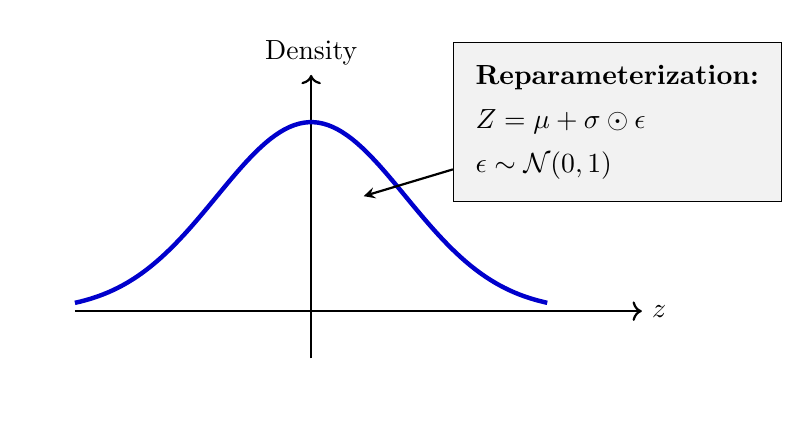
\begin{tikzpicture}[scale=1.2, align=left]
    % Background fill to ensure safe layering
    \fill[white] (-3,-1) rectangle (4,3);
    
    % Axes
    \draw[thick, ->] (-2.5,0) -- (3.5,0) node[right] {$z$};
    \draw[thick, ->] (0,-0.5) -- (0,2.5) node[above] {Density};
    
    % Normal Curve
    \draw[ultra thick, blue!80!black, domain=-2.5:2.5, samples=100] 
        plot (\x, {2*exp(-0.5*\x*\x)});
        
    % Reparameterization Annotation
    \node[black, anchor=west, inner sep=8pt, draw, fill=gray!10] at (1.5, 2) {
        \textbf{Reparameterization:}\\[4pt]
        $\displaystyle Z = \mu + \sigma \odot \epsilon$\\[4pt]
        $\displaystyle \epsilon \sim \mathcal{N}(0,1)$
    };
    
    % Callout arrow
    \draw[->, >=stealth, shorten >=2pt, thick] (1.5, 1.5) -- (0.5, 1.2);
\end{tikzpicture}
\end{center}
\end{proof}

\newpage

\section{Concept Checklist \& Question Mapping (Reference)}

\renewcommand{\arraystretch}{1.5}
\begin{table}[h!]
\centering
\begin{tabularx}{\textwidth}{>{\raggedright\arraybackslash}p{0.3\textwidth} >{\raggedright\arraybackslash}X >{\raggedright\arraybackslash}p{0.2\textwidth}}
\toprule
\textbf{Concept Category} & \textbf{Description \& Techniques} & \textbf{Problem Mapping} \\
\midrule
\textbf{C1: Measure Theory} & Lebesgue measure, dense sets, probability of countable sets, pushforward measures. & 1, 2, 23, 27 \\
\textbf{C2: Uniform Distribution} & CDF derivation, piecewise integration, moments, order statistics. & 5, 7, 21, 22, 28, 29 \\
\textbf{C3: Normal Distribution} & Gaussian integral, inflection points, density maximization. & 6, 11, 12, 23, 24 \\
\textbf{C4: LOTUS} & Law of the Unconscious Statistician, non-linear transformations. & 3, 8, 9, 16 \\
\textbf{C5: Variance \& Moments} & Variance-Moment identity, scaling laws, higher-order moments. & 4, 10, 17, 20 \\
\textbf{C6: Poisson Processes} & Uniform conditioning of arrival times, order statistics. & 15, 20, 21 \\
\textbf{C7: Standardization} & Z-scores, set-theoretic mappings, Normal-Binomial bridging. & 10, 13, 18 \\
\textbf{C8: Transformations} & Jacobians, non-one-to-one mappings, log-normal, chi-square. & 3, 14, 16, 22, 26 \\
\textbf{C9: Diagnostics \& Flaws} & Divergent integrals, Jensen's inequality, point-probability trap. & 2, 4, 15, 24, 25 \\
\textbf{C10: Abstract Modeling} & VAE Reparameterization trick, Black-Scholes log-normal models. & 11, 12, 19, 26, 30 \\
\bottomrule
\end{tabularx}
\end{table}

\end{document}